
\documentclass{article}
\usepackage[utf8]{inputenc}

\title{Laboratorio04_CALIDAD_PRUEBAS_SOFTWARE}
\author{edwartbalcon }
\date{October 2020}

\usepackage[utf8]{inputenc}
\usepackage[spanish]{babel}
\usepackage{natbib}
\usepackage{graphicx}

\begin{document}

\title{Caratula}

\begin{titlepage}
\begin{center}
\begin{Large}
\textbf{UNIVERSIDAD PRIVADA DE TACNA} \\
\end{Large}
\vspace*{-0.025in}
\begin{figure}[htb]
\begin{center}

\includegraphics[width=6cm]{./images/logo_UPT}
\end{center}
\end{figure}
\vspace*{-0.025in}
\begin{Large}
\textbf{FACULTAD DE INGENIERIA} \\
\end{Large}
\vspace*{0.05in}
\begin{Large}
\textbf{Escuela Profesional de Ingeniería de Sistema} \\
\end{Large}


\vspace*{0.1in}

\vspace*{0.1in}
\begin{Large}
\textbf{Informe de laboratorio 05:  Utilizando Desarrollo guiado por comportamiento (BDD)
para realización pruebas de software} \\
\end{Large}

\vspace*{0.3in}
\begin{Large}
\textbf{Curso: Calidad y Pruebas de Software} \\
\end{Large}

\vspace*{0.3in}
\begin{Large}
\textbf{DOCENTE: Ing. Patrick Cuadros Quiroga} \\
\end{Large}

\vspace*{0.2in}
\vspace*{0.1in}
\begin{large}

\begin{Large}
\textbf{Alumno: Balcon Coahila, Edwart Juan\hfill	(2013046516) } \\
\end{Large}

\vspace*{0.15in}
\begin{Large}
\textbf{Tacna – Perú} \\
\end{Large}

\vspace*{0.05in}
\begin{Large}
\textbf{2020 } \\
\end{Large}

\end{large}
\end{center}

\end{titlepage}


\newpage


\textbf{1.Se utilizará el framework CoreBDD. Instalar la plantilla de proyecto dotnet a través de}

    \begin{center}
		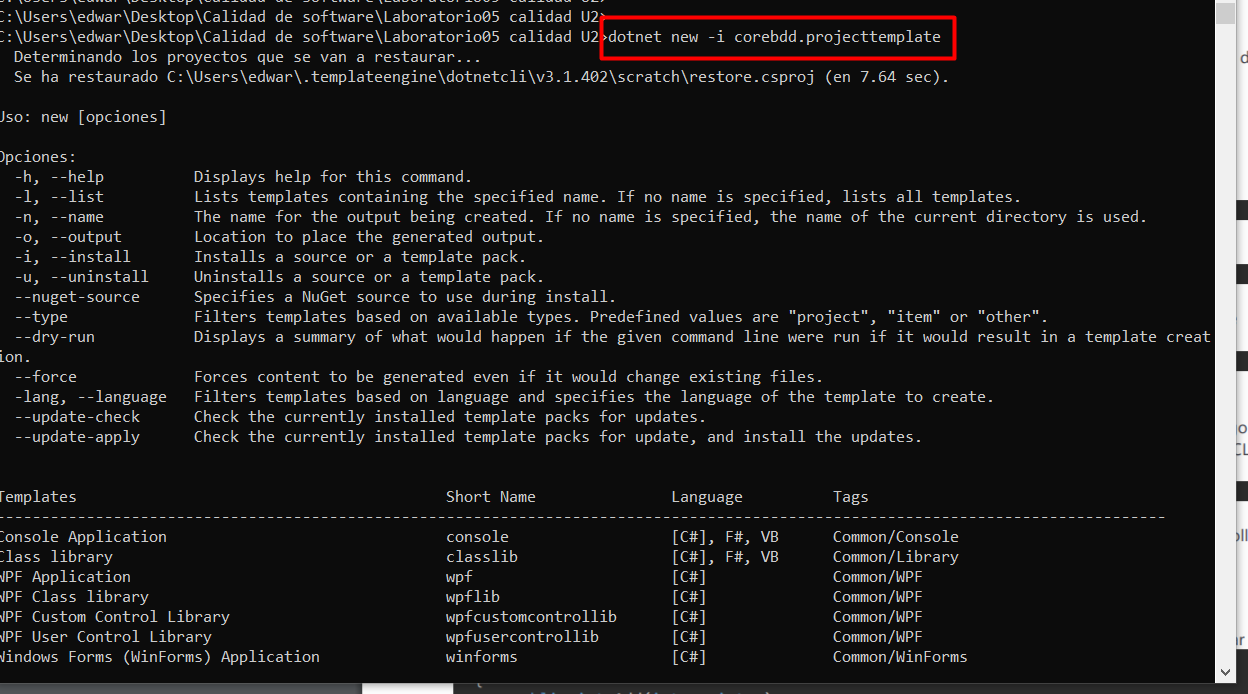
\includegraphics[width=15cm]{./images/1} 
	\end{center}
	
\textbf{2. Luego cree una nueva carpeta para su proyecto de prueba y ejecute
}

    \begin{center}
		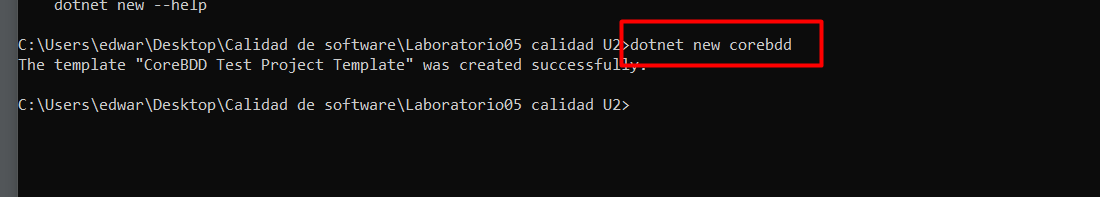
\includegraphics[width=15cm]{./images/2} 
	\end{center}
\newpage
\textbf{3. Alternativamente, puede agregar CoreBDD a un proyecto de prueba xUnit existente a través del paquete
nuget

}

    \begin{center}
		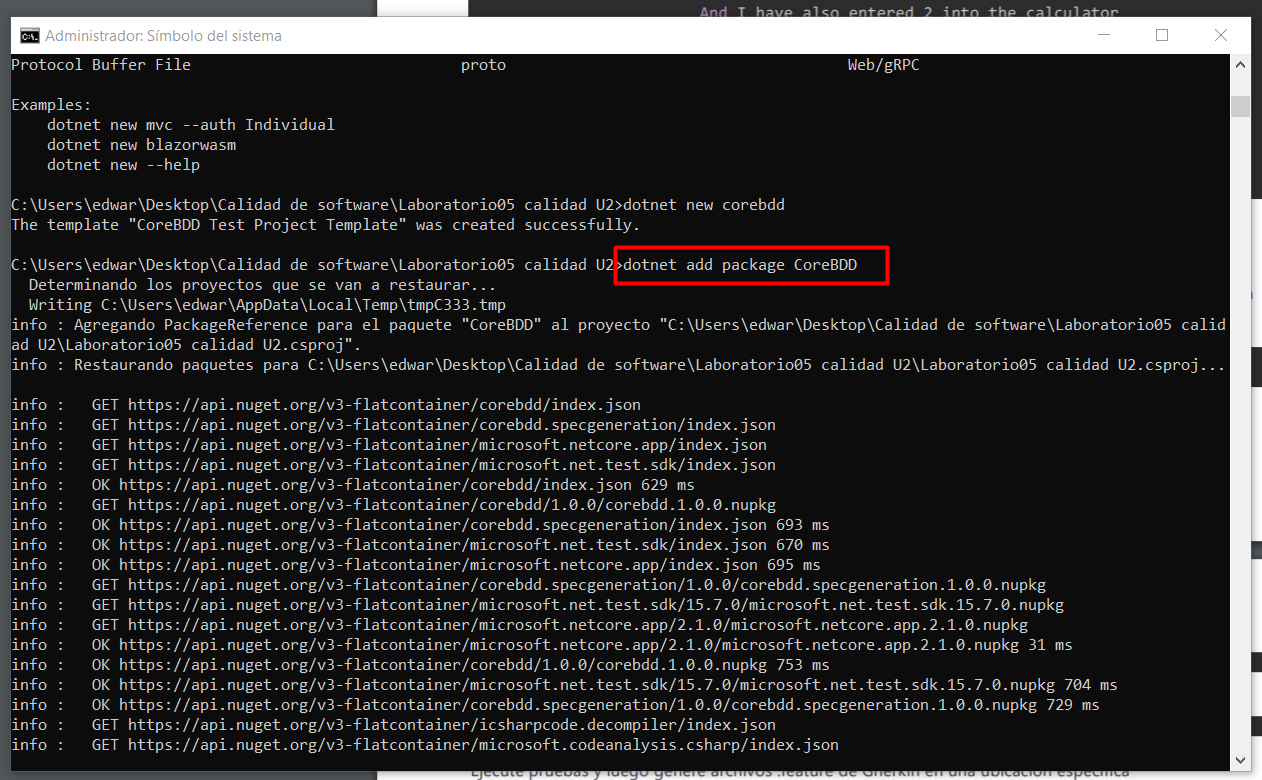
\includegraphics[width=15cm]{./images/3} 
	\end{center}
	\newpage
\textbf{4. La herramienta de línea de comandos facilita la ejecución de tareas como la ejecución de pruebas con la
salida de estilo Gherkin, la generación de archivos de prueba de características y escenarios
predeterminados y la generación de archivos de funciones de Gherkin a partir de pruebas existentes o la
generación de pruebas a partir de archivos de funciones existentes.
Comenzando desde cero usando la plantilla dotnet y las herramientas cli:
}

    \begin{center}
		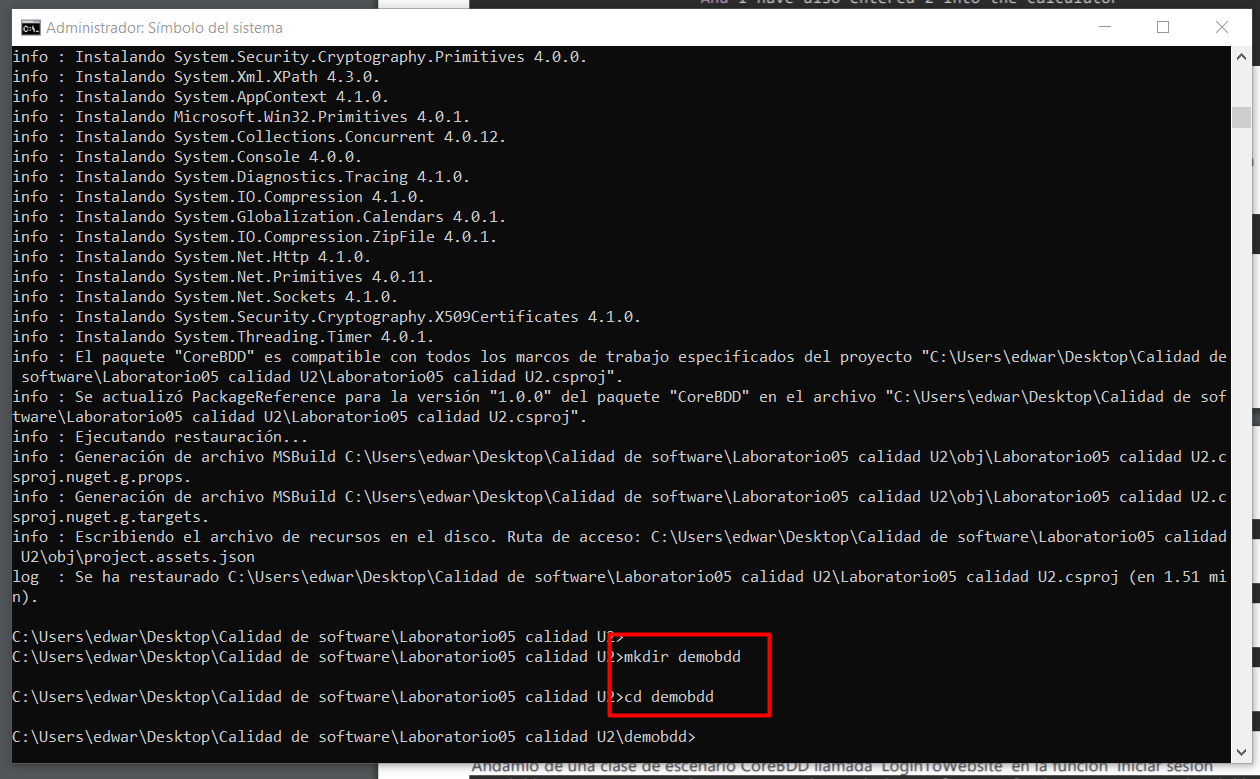
\includegraphics[width=15cm]{./images/4} 
	\end{center}
	
	\textbf{5. Luego cree el nuevo proyecto CoreBDD
}

    \begin{center}
		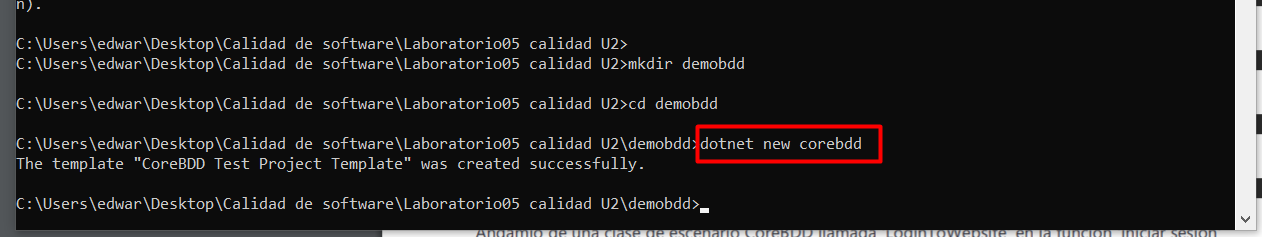
\includegraphics[width=15cm]{./images/5} 
	\end{center}

\end{document}